\documentclass[conference]{IEEEtran}
\IEEEoverridecommandlockouts
% The preceding line is only needed to identify funding in the first footnote. If that is unneeded, please comment it out.
\usepackage{cite}
\usepackage{amsmath,amssymb,amsfonts}
\usepackage{algorithmic}
\usepackage{graphicx}
\usepackage{textcomp}
\usepackage{xcolor}
\def\BibTeX{{\rm B\kern-.05em{\sc i\kern-.025em b}\kern-.08em
    T\kern-.1667em\lower.7ex\hbox{E}\kern-.125emX}}
\begin{document}

\title{Multi-Model Biometric Verification Using Face, Finger and Voice\\
{\footnotesize \textsuperscript{}Improve Security in Android Application using mutli-model biometric}
\thanks{}
}

\author{\IEEEauthorblockN{1\textsuperscript{st} Shashi Saurabh Sinha}
\IEEEauthorblockA{\textit{Computer Science Engineering} \\
\textit{National Institute of Technology Sikkim}\\
Ravangla,Sikkim,India \\
b180043@nitsikkim.ac.in}
\and
\IEEEauthorblockN{2\textsuperscript{nd} Dr. Pankaj Kumar Keserwani}
\IEEEauthorblockA{\textit{ Assistant Professor}\\  \textit{ Departement of Computer Science Engineering} \\
\textit{National Institute of Technology Sikkim}\\
Ravangla,Sikkim,India \\
pankajkeserwani.cse@nitsikkim.ac.in}
\and
\IEEEauthorblockN{3\textsuperscript{rd} Kiran Gajjana}
\IEEEauthorblockA{\textit{Computer Science Engineering} \\
\textit{NIT Sikkim}\\
Ravangla,Sikkim,India \\
m210008@nitsikkim.ac.in}
}

\maketitle

\begin{abstract}
For many years, people have seen one other in various ways. When we meet people, we see them through their looks and hear them through their voices. In computer systems, verification (authentication) is usually dependent on an individual's ownership (key, magnet, or chip card) or personal information (PIN, password). Keys and cards, on the other hand, are often stolen or lost, while passwords are frequently forgotten or exposed. The advantages of biometric authorization are that it requires the user to be there and avoids the inconveniences of passwords and PINs. 

The goal of our project is to create a multi-model biometric verification system that could successfully validate a person's identification by matching the scanned fingerprint ,matching  face and  matching voice at same time. The project's purpose is to build and improve the whole computational element of the fingerprint and face verification and voice verification processes on Android  for ultimate deployment in a real-time online system. In this paper discusses how we developed this system and then analyses the outcomes.
\end{abstract}

\begin{IEEEkeywords}
Face verificaton,Fingerprint verification,Voice verification,Multi-Model Biometric, Android
\end{IEEEkeywords}

\section{Introduction}
Biometric verification has often been recognized as the most trust proof, or at the very least the most difficult to fake or spoof. Diagnostic and verification systems have been physically based aspects in the IT industry since the early 1980s. These biometric methods were sluggish, intrusive, and repetitively costly, but they seem to function in certain high-security circumstances since they were frequently employed to monitor access to vast frames or visual constraints logging in to a few people again and over again. Computers are now lot quicker and less expensive than they were twenty years ago. This, along with new, low-cost gear, has rekindled interest in biometrics.

Identify theft and management or disclosure of data and intellectual property connected to increasing concerns in this computer-driven world. We all have several accounts and use a large number of passwords on an increasing number of machines and websites. It is getting more challenging to maintain and manage access while securing both user identification and computer data and systems. The principle of authentication, which guarantees the user is who they say they are, is fundamental to all security.

To get more trustworthy verification or identification, we must employ something that accurately portrays the individual. Biometrics offers automated techniques of authenticating identity or identify based on quantifiable or behavioural attributes such as fingerprints, voice, or facial recognition. Features are quantifiable and distinct. These characteristics should not be duplicated, but it is frequently easy to generate a clone that the biometric system accepts as the original sample. This is a frequent circumstance in which the degree of protection given is determined by the amount of money required by the fraudster to get unauthorized access.

Biometric data is individual private information that is uniquely and permanently connected with a person and, unlike credentials or keys, could be changed. Once an opponent breaches a user's biometric data, the data is gone permanently, perhaps resulting in a large financial loss. As a result, one key problem is how to preserve a person's biometric data after it has been gathered

\section{Problem Definition}

\subsection{Problem With Previous system}

We live in digital world and everyone using smartphone and other electronic device. All work is going to
shift in digital.As digital/online data increasing day by day and in parallel online farud is also
growing.Everyone Concern about privacy and secure your data from fraud activity.In recent time data vulnerability/data leak has increase.Credentail like
(pin,Password,username,credit card details,tokenid etc) are present in dark web.Anyone can access
their data.There is problem with one factor authentication that it can be eaisly hacked and it is forgetten by user.Problem with two factor is that it can be stolen or forgetten.Diagnose based on a single biometric component may be insufficient and has limited capacity to detect fraud.All type of authentication are not secure to preserve the data and authenticate the right person.So we purpose the biometric Authentication. Every person has unique biological characteristics.But problem in prsent system is that we verify single-single biometric at one-time.So
it can also be faked by using the captured image,recorded voice,Match fingerpint sample. Because of non-standard biometric characteristics, biometric authentication systems often have registration issues. poor precision due by noisy data gathering in specific locations Because of environmental noise, signal distortion, changes in biometric traits, and variability, biometric readings fluctuate naturally.
\section{Propose Model}

The term biometrics comes from the Greek words bio and metric. The phrase Bio refers to Physical characteristic and metric refer to identification.All person has different physical characteristic so we can eaisly authenticate a person and minimize the farud with the combination of more than one biometric characteristic.So we
purpose the authentication model which take all three type of data at one time and match with template.If anyone of not match with template then system not verify the person. Person verifed
only if all the biometric charactersistic matched.we improve the security system. In this we use finger, face and voice characteristic to verify the person. We give the option to user for enable three factor biometric authentication while signup or signin into the application. User can directly login with email and password or use their biometric to login or signup into the application.

\subsection{Methodolgy}\label{AA}
When user Open the application then we give option to the user for signup and Sigin. We also give the option to the user for biometric enable or disable.If user disable the biometric then user can sigin/sigup using email and password.If user enable the biometric then we take biometric data at the time of sigup. After taking the biometric data check the quality of biometric data. if it sufficient then we generate the template otherwise collect again.we collect the image from camera, collect fingerprint using sensor and collect voice using mic.
\linebreak

{\bf A biometric system typically has four major components.}
\begin{itemize}
	\item Well how scan and capture a digital edition of a live unique biometric element.
	\item Raw data processing software is converted into a format (referred to as a template) that may be used either storage and matching.
	\item Being software that compares a pre-stored biometric data to a live example template.
	\item A visual interface for communicating the match impact with the app.
	
\end{itemize}

\subsection{Methodogoly for face verification}
In this i use CNN model for the face verification which give the more accuracy.The model structure is divided into 5 model,all model different in some parameters like network width,input data.This model composed of two convolution layers and two pooling layers and all these layer are alternatively arranged.Input layer has only one feature map,and it is used to add normalized face picture into the CNN model.Convolutional layer which contains six feature maps where each neuron is convoluted with a completely random convolution kernel of size 5x5.Pooling layer which has output is six feature maps computed based on the preceding layer's output. Each element in the feature map is linked to the average convolution kernel of the corresponding feature map in covolution layer.Using Cnn we generate the template and stored in database at the time of user signup.When user login then we matched template which stored in database.It it matched then user is verified.
\subsection{Methodology for Fingerprint Verificaton}
We must first get digital fingerprints before proceeding.Fingerprints are not similar and are seldom saved as bitmaps. There are two types of fingerprint matching strategies: minutiae-based and communication-based.
Minutiae-based strategies first locate minutiae points and then map out their associated location placement. Minutiae are distinguishing characteristics of a fingerprint pattern, such as hind ends, double splits, splits, dots, or islands (see photo on next page).We generate template and stored in database in time of sigup.When user login then verify the fingerprint with stored template in database.if matched then user is verified.
\subsection{Methodology for Voice Verificaton}
Speech recognition is a technique that allows a phone to capture human speech using a microphone. A speech impairment later detects these words, and the system finally releases recognisable terms. The voice recognition process consists of many processes.In this we use google api to convert human voice to word and stored in database as a secret key. When user sigin then it speak secrect word which is matched with database data. if matched then user is verifed.

\section{Sequence Diagram Use Case FlowChart Result}
\begin{figure}[htbp]
	\centerline{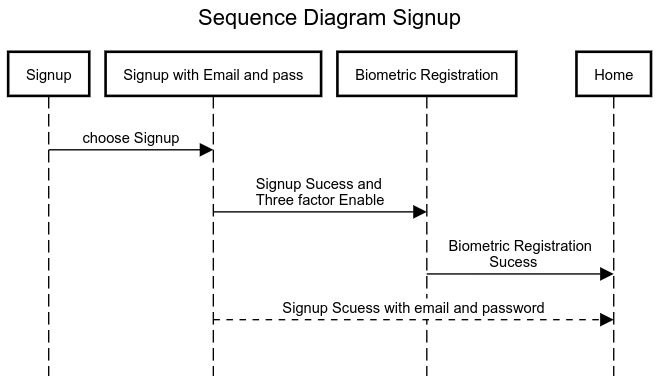
\includegraphics[width=1.0\columnwidth]{sequp.png}}
	\caption{Signup Sequence Diagram}
	\label{fig}
\end{figure}
\begin{figure}[htbp]
	\centerline{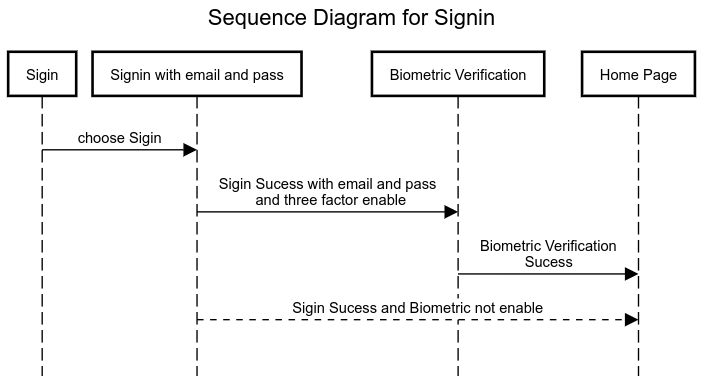
\includegraphics[width=1.0\columnwidth]{seqin.png}}
	\caption{Signinp Sequence Diagram}
	\label{fig}
\end{figure}
\begin{figure}[htbp]
	\centerline{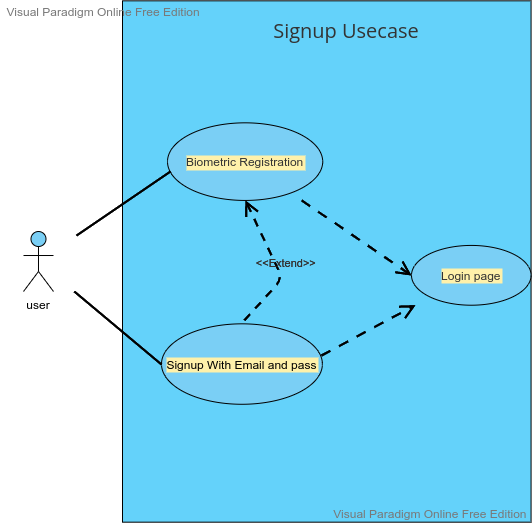
\includegraphics[width=1.0\columnwidth]{useup.png}}
	\caption{Sigup Use Case}
	\label{fig}
\end{figure}
\begin{figure}[htbp]
	\centerline{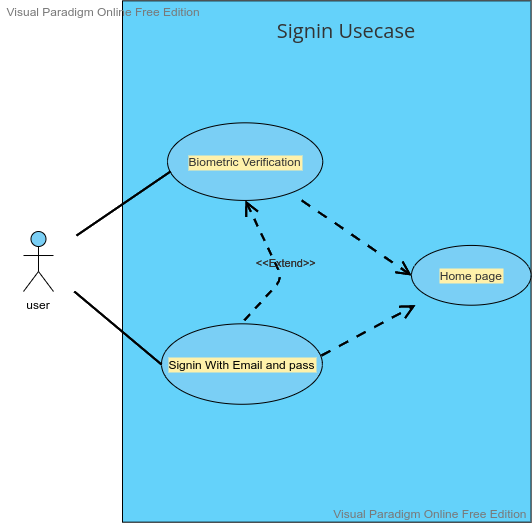
\includegraphics[width=1.0\columnwidth]{usein.png}}
	\caption{Sigin Use Case}
	\label{fig}
\end{figure}

\begin{figure}[htbp]
	\centerline{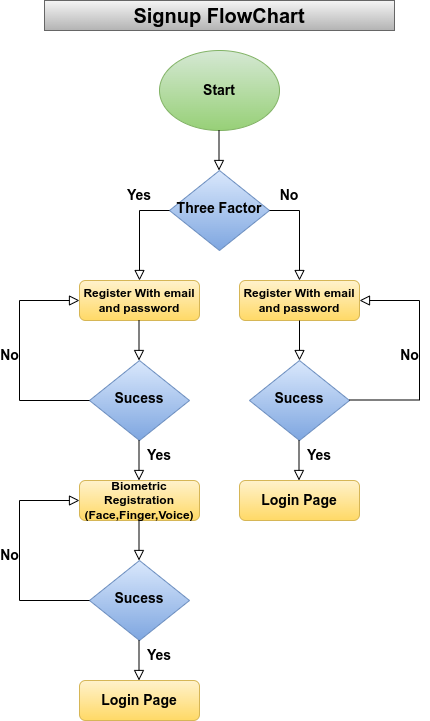
\includegraphics[width=0.8\columnwidth]{signup.png}}
	\caption{SignUp Flow Chart }
	\label{fig}
\end{figure}
\begin{figure}[htbp]
	\centerline{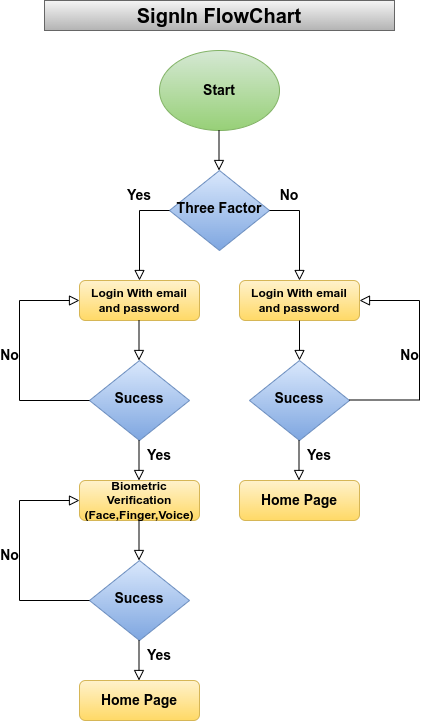
\includegraphics[width=.8\columnwidth]{sigin.png}}
	\caption{Signin Flow Chart }
	\label{fig}
\end{figure}
\begin{figure}[htbp]
	\centerline{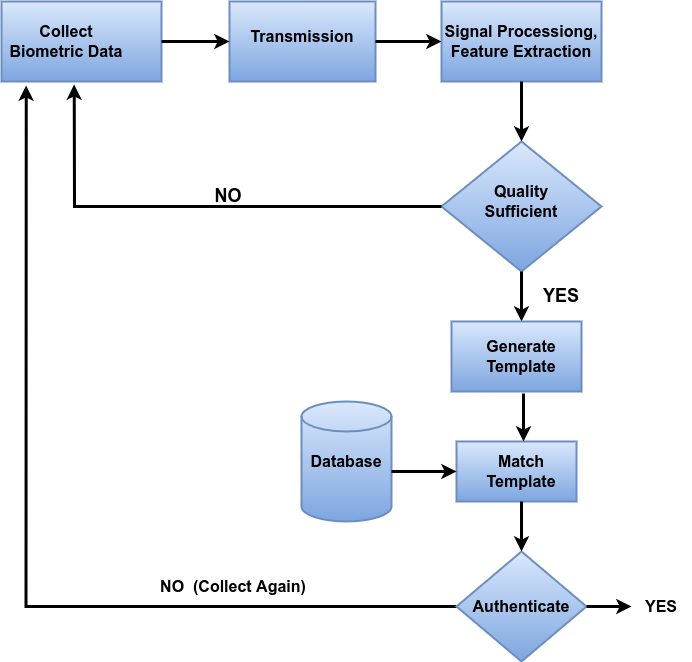
\includegraphics[width=1.0\columnwidth]{metho.png}}
	\caption{Methodology for Biometric }
	\label{fig}
\end{figure}
\begin{figure}[htbp]
	\centerline{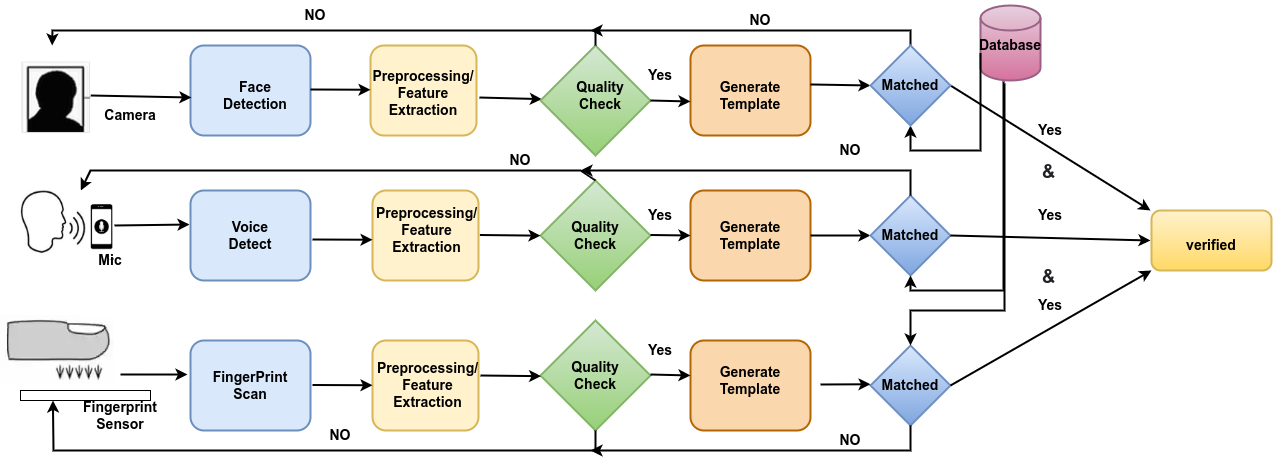
\includegraphics[width=1.0\columnwidth]{biometric.png}}
	\caption{biometric Verificaton }
	\label{fig}
\end{figure}


\begin{figure}[htbp]
	\centerline{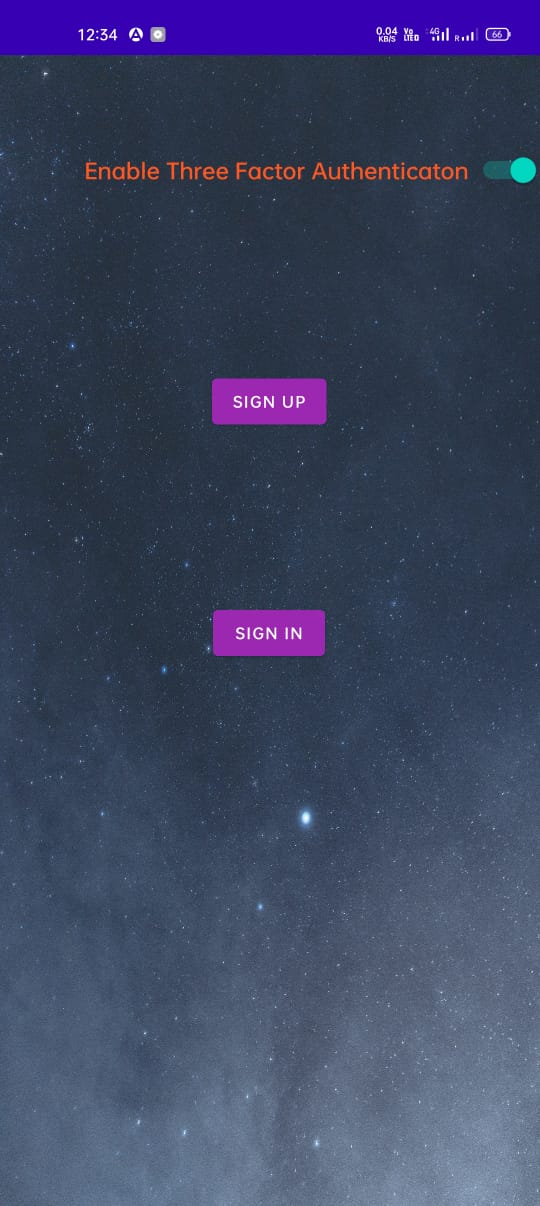
\includegraphics[width=0.4\columnwidth]{signupbiometric.jpeg}}
	\caption{Sigin/Signup With Biometric enable }
	\label{fig}
\end{figure}
\begin{figure}[htbp]
	\centerline{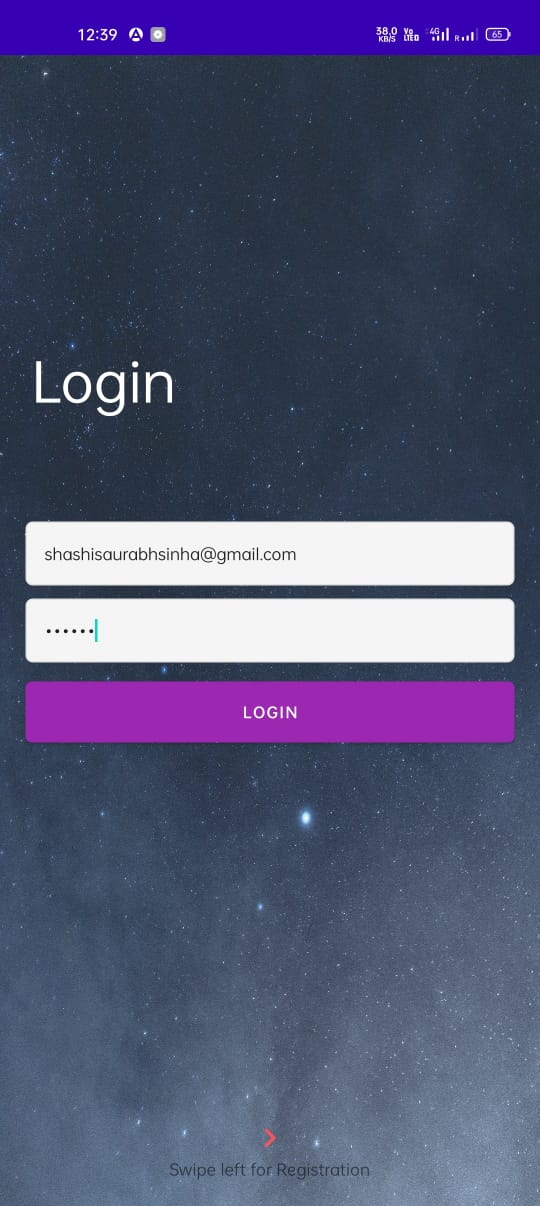
\includegraphics[width=0.4\columnwidth]{emaillog.jpeg}}
	\caption{Login With Email and password}
	\label{fig}
\end{figure}
\begin{figure}[htbp]
	\centerline{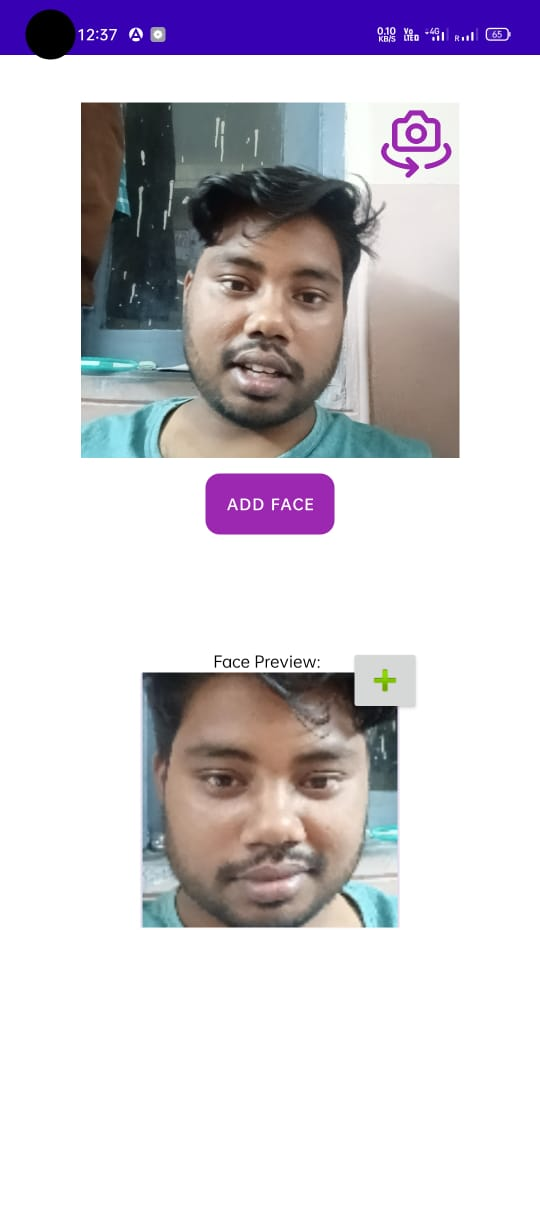
\includegraphics[width=0.4\columnwidth]{enrollface.jpeg}}
	\caption{Enroll Face }
	\label{fig}
\end{figure}
\begin{figure}[htbp]
	\centerline{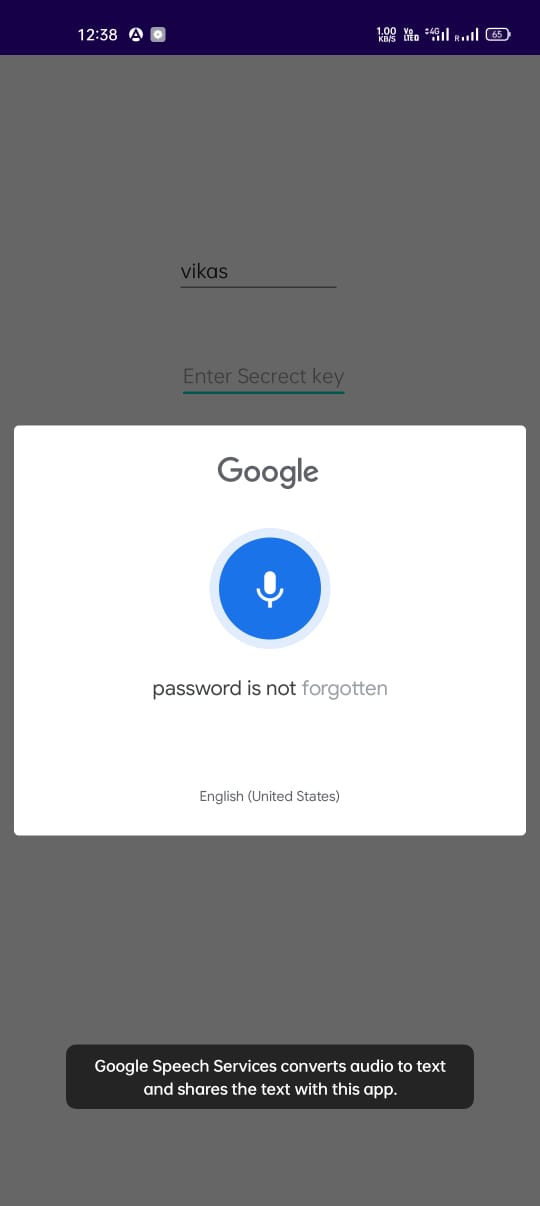
\includegraphics[width=0.4\columnwidth]{enrollvoice.jpeg}}
	\caption{Enroll Voice}
	\label{fig}
\end{figure}
\begin{figure}[htbp]
	\centerline{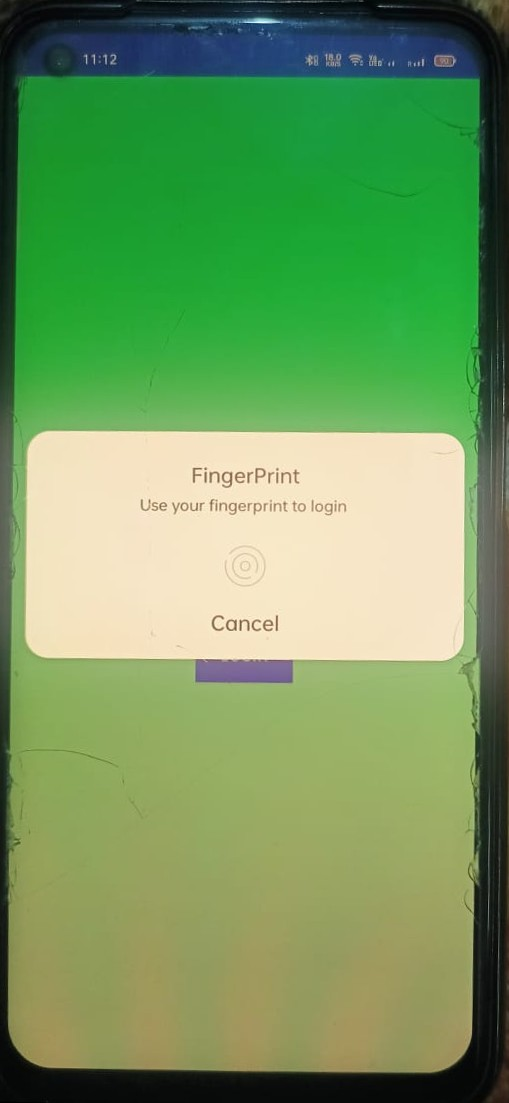
\includegraphics[width=0.4\columnwidth]{finger.jpeg}}
	\caption{Finerprint Enroll }
	\label{fig}
\end{figure}
\begin{figure}[htbp]
	\centerline{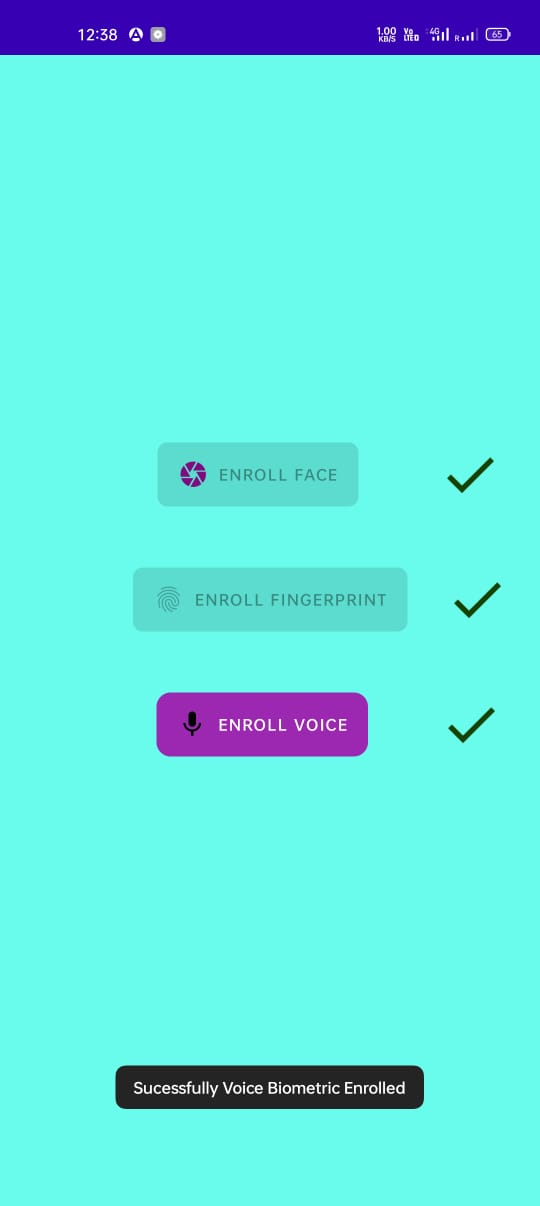
\includegraphics[width=0.4\columnwidth]{sucesenrollall.jpeg}}
	\caption{Sucessfully Enroll all Biometric}
	\label{fig}
\end{figure}
\begin{figure}[htbp]
	\centerline{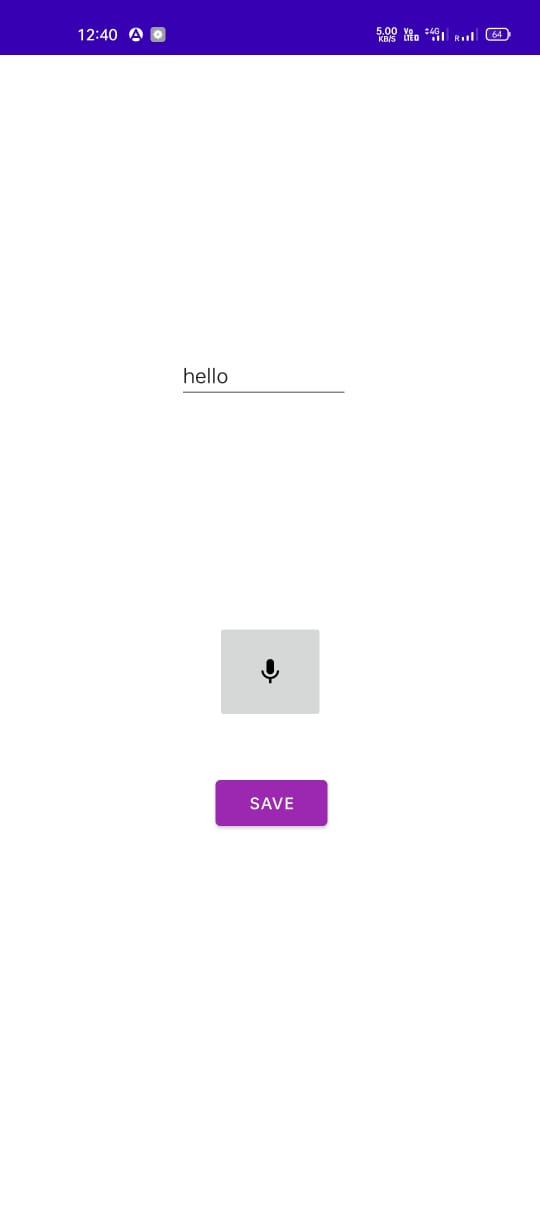
\includegraphics[width=0.4\columnwidth]{verifyvoice.jpeg}}
	\caption{Verify Voice }
	\label{fig}
\end{figure}
\begin{figure}[htbp]
	\centerline{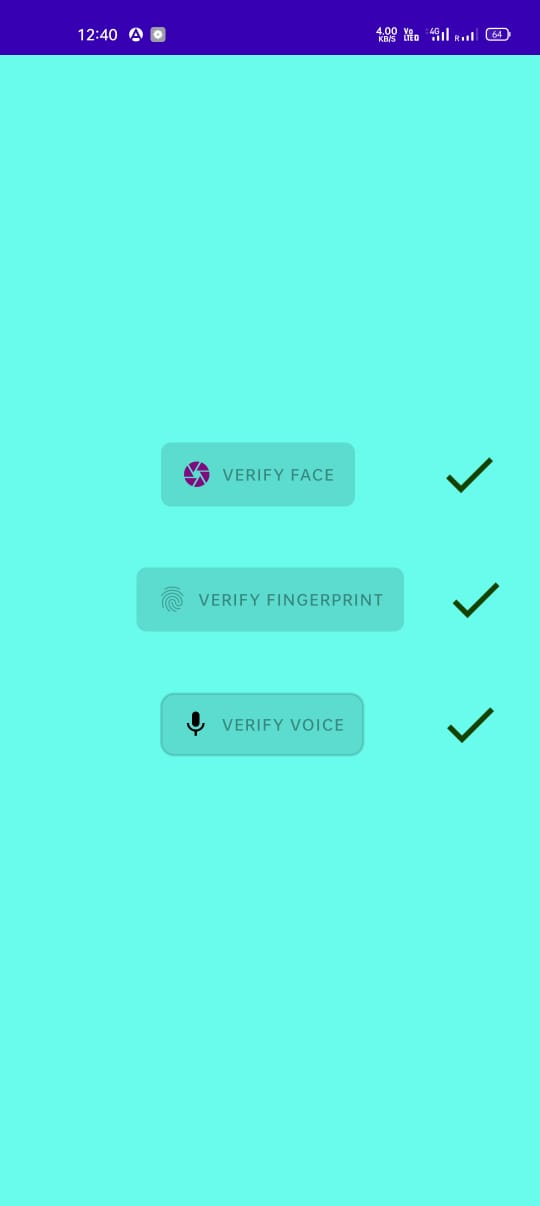
\includegraphics[width=0.4\columnwidth]{allverify.jpeg}}
	\caption{All Verified }
	\label{fig}
\end{figure}
\begin{figure}[htbp]
	\centerline{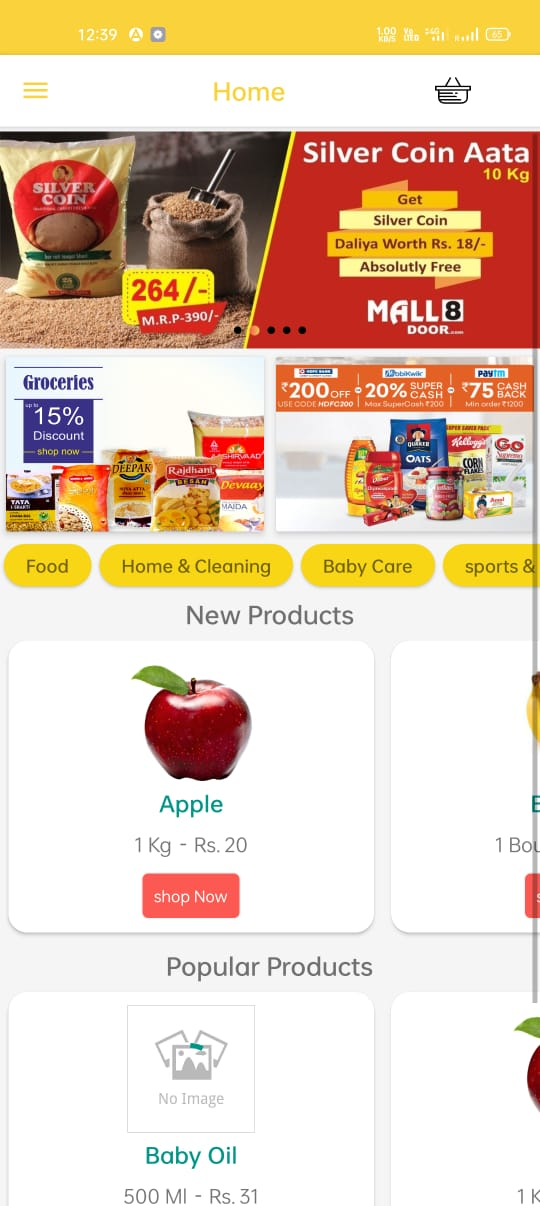
\includegraphics[width=0.4\columnwidth]{Homepage.jpeg}}
	\caption{Home page Grocery Shop }
	\label{fig}
\end{figure}
\begin{figure}[htbp]
		
		\centerline{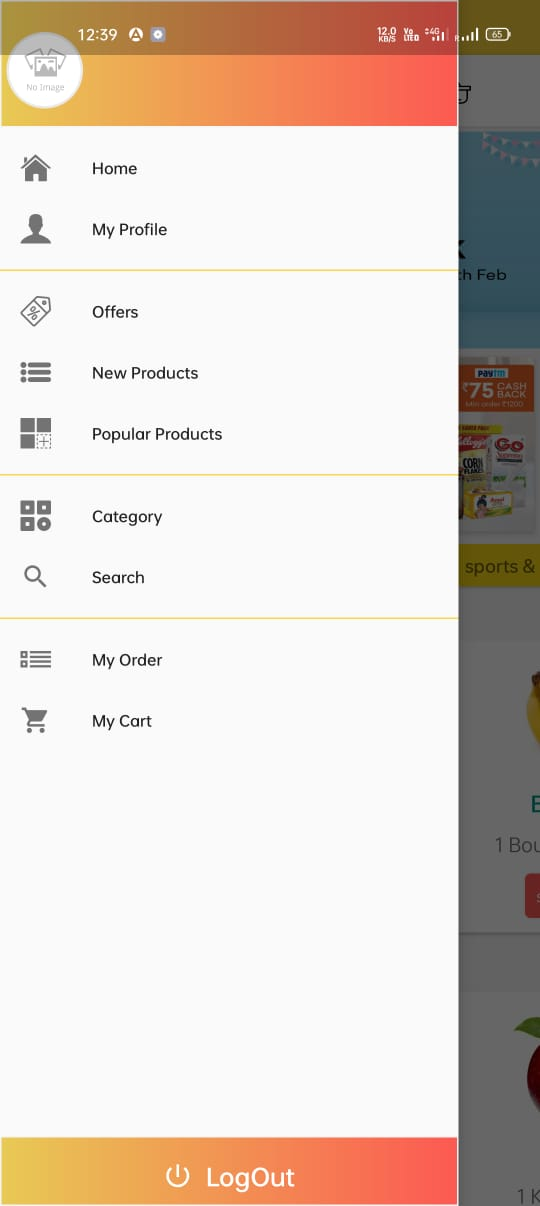
\includegraphics[width=0.4\columnwidth]{homepage2.jpeg}}
		\caption{Profile and Logout page }
		\label{fig}
\end{figure}


\afterpage{\clearpage}
\section{Conclustion}
We have sucessfully build three factor biometric authentication application which veriy the finger, face and voice given by the user and secure the application being fraud.we use built camra for face verify, fingerprint sensor to verify the user fingerprint and use mic for voice verification.First we enroll the user by email and password after this we enroll for the biometric. When user login into the application we verify the biometric characteristic of user and allow user to login into the application.
\subsection{Advantage}
\begin{itemize}
	\item It make system more Secure.Anyone can’t easily fake this system.
	\item It is best option to verify the unskilled person with the biometric characteristic.
	\item The combination of all three biometric increase the effectivness of the verfication.
	\item if acceptability is taken into account. It mean that it is verfied person.
\end{itemize}
\subsection{Disadvantage}
\begin{itemize}
	\item It take more time to verfiy a person than any of individual verfication.
	\item It require more hardware component to verify the person.
	\item It is costlier than other verifcation system.
	\item Sometime it create problem when person changed face due to some accident or other
	situation.Change in fingerprint due to cut in finger or any accident. Change in Voice of due to
	illness or some change in vocal voice
	\item It require more time to enroll the people.
	\item It require more database to store the template and also require more computing power for verify.
	\item It may not applicable for voiceless person.
	\item It may not applicable for the person which has not fingerprint in his hand.
\end{itemize}
\section{Future Work}
Given that the most significant shortcoming in the existing implementation of this project is the lack of speed, that would be the top priority of any changes. Reducing the runtime of a single experiment from  minutes to less than few second.

{\bf The following are the upcoming works:}

1. We will implement this on other device providing a high level of security.

2. Make biometric verification more secure so that it cannot be easily faked.

3. Introduce another form of biometric verification that can aid in its detection. If one of the methods fails, such as the heart-bit, DNA verification can be used to validate.


4. Biometrics System- Face Recognition is on the verge of becoming more advanced. Security limitations are required for almost any software. We intend to replace traditional security constraint approaches with Biometrics Systems—Face Recognition, Voice Identification, or both.

5. We will imporve the database protection and use blockchain to protect database.


\section*{Acknowledgment} I am tremendously indebted to my supervisor {\bf Dr. Pankaj Kumar Keserwani}, Assistant Professor , Department of Computer Science and Engineering, National Institute of Technology Sikkim for his invariable guidance and assistance throughout the project. His advice and suggestions have been prized in the development and progress of the content. Furthermore, the skills and knowledge which I have gained throughout this project I perceive as very valuable and significant for my future. I take this opportunity to acknowledge all professors and research scholars who have provided their valuable experience throughout this entire curriculum and led to my piece-meal growth as a student. Finally, I express my deepest gratitude to my family and friends for their untiring encouragement and unconditional support.
\section*{}
\begin{thebibliography}{00}
\bibitem{b1} Prasad Pawar 1 , Shreyas Datar 2 , Nilay Ranade 3 , Kunal Thorat 4 , Prof.A.N.Gharu 5(2019),Biometric Security Using Cryptography for Insurance
\bibitem{b2} International Journal of Recent Technology and Engineering (IJRTE) ,Mohammed, Bayan Omar. "Mean-Discrete Algorithm for Individuality Representation." Journal of Al-Qadisiyah for computer science and mathematics 13, no. 1 (2021).
\bibitem{b3} Al-Nima, R.R.O., Abdullah, M.A., Al-Kaltakchi, M.T., Dlay, S.S., Woo, W.L. and Chambers, J.A., 2017. Finger texture biometric verification exploiting multi-scale sobel angles local binary pattern features and score-based fusion. Digital Signal Processing, 70, pp.178-189.
\bibitem{b4} de Freitas Pereira, T. and Marcel, S., 2021. Fairness in biometrics: a figure of merit to assess biometric verification systems. IEEE Transactions on Biometrics, Behavior, and Identity Science, 4(1), pp.19-29.
\bibitem{b5} Sawhney, S., Kacker, K., Jain, S., Singh, S.N. and Garg, R., 2019, January. Real-time smart attendance system using face recognition techniques. In 2019 9th International Conference on Cloud Computing, Data Science and Engineering (Confluence) (pp. 522-525). IEEE.
\bibitem{b6} Kaur, N., 2021, March. A study of biometric identification and verification system. In 2021 International Conference on Advance Computing and Innovative Technologies in Engineering (ICACITE) (pp. 60-64). IEEE.
\bibitem{b7} Ibrahim, S., Egila, M.G., Shawky, H., Elsaid, M.K., El-Shafai, W., El-Samie, A. and Fathi, E., 2020. Cancelable face and fingerprint recognition based on the 3D jigsaw transform and optical encryption. Multimedia Tools and Applications, 79(19), pp.14053-14078.
\bibitem{b8} Kaur, N., 2021, March. A study of biometric identification and verification system. In 2021 International Conference on Advance Computing and Innovative Technologies in Engineering (ICACITE) (pp. 60-64). IEEE.
\bibitem{b9} Połap, D. and Woźniak, M., 2018. Voice recognition by neuro-heuristic method. Tsinghua Science and Technology, 24(1), pp.9-17.
\bibitem{b10} Herbadji, A., Guermat, N., Ziet, L. and Cheniti, M., 2019, November. Multimodal Biometric Verification using the Iris and Major Finger Knuckles. In 2019 International Conference on Advanced Electrical Engineering (ICAEE) (pp. 1-5). IEEE.
\bibitem{b11} Alarifi, A., Amoon, M., Aly, M.H. and El-Shafai, W., 2020. Optical PTFT asymmetric cryptosystem-based secure and efficient cancelable biometric recognition system. IEEE Access, 8, pp.221246-221268.
\bibitem{b12} Natgunanathan, I., Mehmood, A., Xiang, Y., Beliakov, G. and Yearwood, J., 2016. Protection of privacy in biometric data. IEEE access, 4, pp.880-892.
\bibitem{b13} M. Arsenovic, S. Sladojevic, A. Anderla, and D. Stefanovic, “FaceTime - Deep learning based
\bibitem{b14} ace recognition attendance system,” SISY 2017 - IEEE 15th Int. Symp. Intell. Syst. Informatics,Proc., pp. 53–57, 2017
\end{thebibliography}


\end{document}
